\pdfminorversion=4
\documentclass[10pt]{beamer}\usepackage[]{graphicx}\usepackage[]{color}
%% maxwidth is the original width if it is less than linewidth
%% otherwise use linewidth (to make sure the graphics do not exceed the margin)
\makeatletter
\def\maxwidth{ %
  \ifdim\Gin@nat@width>\linewidth
    \linewidth
  \else
    \Gin@nat@width
  \fi
}
\makeatother

\definecolor{fgcolor}{rgb}{0.345, 0.345, 0.345}
\newcommand{\hlnum}[1]{\textcolor[rgb]{0.686,0.059,0.569}{#1}}%
\newcommand{\hlstr}[1]{\textcolor[rgb]{0.192,0.494,0.8}{#1}}%
\newcommand{\hlcom}[1]{\textcolor[rgb]{0.678,0.584,0.686}{\textit{#1}}}%
\newcommand{\hlopt}[1]{\textcolor[rgb]{0,0,0}{#1}}%
\newcommand{\hlstd}[1]{\textcolor[rgb]{0.345,0.345,0.345}{#1}}%
\newcommand{\hlkwa}[1]{\textcolor[rgb]{0.161,0.373,0.58}{\textbf{#1}}}%
\newcommand{\hlkwb}[1]{\textcolor[rgb]{0.69,0.353,0.396}{#1}}%
\newcommand{\hlkwc}[1]{\textcolor[rgb]{0.333,0.667,0.333}{#1}}%
\newcommand{\hlkwd}[1]{\textcolor[rgb]{0.737,0.353,0.396}{\textbf{#1}}}%

\usepackage{framed}
\makeatletter
\newenvironment{kframe}{%
 \def\at@end@of@kframe{}%
 \ifinner\ifhmode%
  \def\at@end@of@kframe{\end{minipage}}%
  \begin{minipage}{\columnwidth}%
 \fi\fi%
 \def\FrameCommand##1{\hskip\@totalleftmargin \hskip-\fboxsep
 \colorbox{shadecolor}{##1}\hskip-\fboxsep
     % There is no \\@totalrightmargin, so:
     \hskip-\linewidth \hskip-\@totalleftmargin \hskip\columnwidth}%
 \MakeFramed {\advance\hsize-\width
   \@totalleftmargin\z@ \linewidth\hsize
   \@setminipage}}%
 {\par\unskip\endMakeFramed%
 \at@end@of@kframe}
\makeatother

\definecolor{shadecolor}{rgb}{.97, .97, .97}
\definecolor{messagecolor}{rgb}{0, 0, 0}
\definecolor{warningcolor}{rgb}{1, 0, 1}
\definecolor{errorcolor}{rgb}{1, 0, 0}
\newenvironment{knitrout}{}{} % an empty environment to be redefined in TeX

\usepackage{alltt}
%% O comando acima foi necessario porque o PDF nao abria no acrobat do
%% windows, dava o erro 131. Provavelmente devido as figuras em
%% PDF. Agora ele gera um PDF versao 1.4, ao inves da versao 1.5

\usetheme[compress]{PaloAlto}
\usecolortheme{sidebartab} % crane

\usepackage[brazilian]{babel}
\usepackage[T1]{fontenc}
\usepackage[utf8]{inputenc}
\usepackage{graphicx}
\usepackage{hyperref}
\usepackage[scaled]{beramono} % truetype: Bistream Vera Sans Mono
%\usepackage{inconsolata}
\usepackage{amsmath}
\usepackage{xfrac}
\usepackage{tikz}
\usepackage{xcolor}
\usepackage{multirow}
\usepackage{multicol}
\usepackage{tikz}
\usetikzlibrary{arrows, decorations.pathmorphing, backgrounds, fit,
  positioning, calc, trees, plotmarks}

\setbeamertemplate{footline}[frame number] % mostra o numero dos slides
\setbeamertemplate{navigation symbols}{} % retira a barra de navegacao

\usepackage{xspace}
\providecommand{\eg}{\textit{e.g.}\xspace}
\providecommand{\ie}{\textit{i.e.}\xspace}
\providecommand{\R}{\textsf{R}\xspace}
\newcommand{\mb}[1]{\mathbf{#1}}
\newcommand{\bs}[1]{\boldsymbol{#1}}
\providecommand{\E}{\text{E}}
\providecommand{\Var}{\text{Var}}
\providecommand{\DP}{\text{DP}}
\providecommand{\EP}{\text{EP}}
\providecommand{\N}{\text{N}}
\theoremstyle{definition}
\newtheorem*{mydef}{Definição}
\newtheorem*{mythm}{Teorema}

\title{Estimação pontual e distribuições amostrais}
\author[]{Fernando de Pol Mayer}
\institute[UFPR]{Laboratório de Estatística e Geoinformação (LEG) \\
  Departamento de Estatística (DEST) \\
  Universidade Federal do Paraná (UFPR)}
\date{}
\logo{
\includegraphics[width=1.6cm]{../img/ufpr-logo.png}}
\titlegraphic{
\includegraphics[width=1cm]{../img/CC_by-nc-sa_88x31.png}\\
  \tiny
  \href{https://creativecommons.org/licenses/by-nc-sa/4.0/deed.pt_BR}{Este
    conteúdo está disponível por meio da Licença Creative Commons 4.0
    (Atribuição/NãoComercial/PartilhaIgual)}}

\AtBeginSection[]
{
  \begin{frame}
    \frametitle{Plano de aula}
    \tableofcontents[currentsection]
  \end{frame}
}

\AtBeginSubsection[]
{
  \begin{frame}
    \frametitle{Plano de aula}
    \tableofcontents[currentsection,currentsubsection]
  \end{frame}
}
\IfFileExists{upquote.sty}{\usepackage{upquote}}{}
\begin{document}





\begin{frame}
\maketitle
%\titlepage
\end{frame}

\begin{frame}{Sumário}
\tableofcontents
\end{frame}

\section[Introdução]{Introdução}

\begin{frame}{Inferência estatística}
\begin{mydef}[Inferência estatística]
  Seja $X$ uma variável aleatória com função densidade (ou de
  probabilidade) denotada por $f(x,\theta)$, em que $\theta$ é um
  parâmetro desconhecido. Chamamos de \textbf{inferência estatística} o
  problema que consiste em especificar um ou mais valores para $\theta$,
  baseado em um conjunto de valores $X$.
  \end{mydef}
  \vspace{1em}
  A inferência pode ser feita através de duas formas:
  \begin{itemize}
  \item estimativa pontual
  \item estimativa intervalar
  \end{itemize}
\end{frame}

\begin{frame}{Inferência estatística}
  \textbf{Redução de dados} \\~\\

  Um experimentador usa as informações em uma amostra aleatória $X_1,
  \ldots, X_n$ para se fazer inferências sobre $\theta$. \\~\\
  Normalmente $n$ é grande e fica inviável tirar conclusões baseadas em
  uma longa \textbf{lista} de números. \\~\\
  Por isso, um dos objetivos da inferência estatística é \textbf{resumir} as
  informações de uma amostra, da maneira mais \textbf{compacta}
  possível, mas que ao mesmo tempo seja também
  \textbf{informativa}. \\~\\
  Normalmente esse resumo é feito por meio de \textbf{estatísticas}, por exemplo,
  a média amostral e a variância amostral.
\end{frame}

\begin{frame}{População e amostra}
  \begin{mydef}[População]
    O  conjunto de valores de uma característica associada a uma coleção
    de indivíduos ou objetos de interesse é dito ser uma população.
  \end{mydef}

  \begin{mydef}[Amostra]
    Uma sequência $X_1, \ldots, X_n$ de $n$ variáveis aleatórias
    independentes e identicamente distribuídas (iid) com função
    densidade (ou de probabilidade) $f(x,\theta)$ é dita ser uma amostra
    aleatória de tamanho $n$ da distribuição de $X$. Como normalmente
    $n>1$, então temos que a fdp ou fp conjunta será
    \begin{equation*}
      f(\bs{x, \theta}) = f(x_1, \ldots, x_n, \theta) = \prod_{i=1}^n
      f(x_i, \theta)
    \end{equation*}
  \end{mydef}
\end{frame}

\begin{frame}{População e amostra}
  \begin{figure}[h]
    \centering
    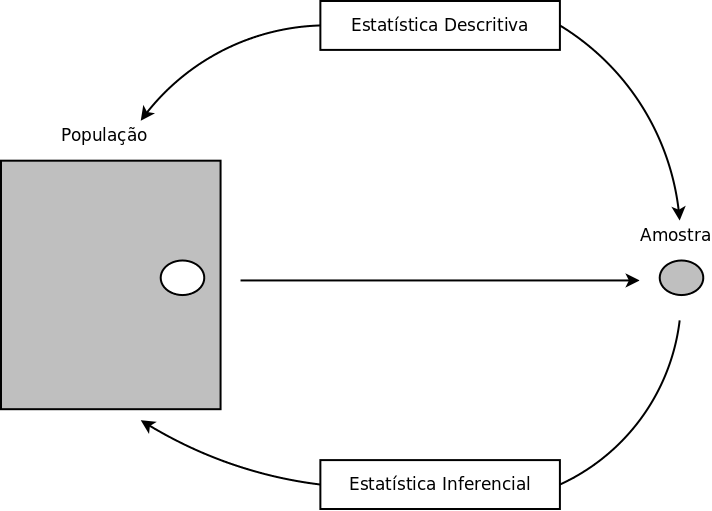
\includegraphics[width=.9\textwidth]{../img/populacao_amostra.png}
  \end{figure}
\end{frame}

\begin{frame}{Parâmetro e Estatística}
  \begin{center}
    População $\rightarrow$ \textbf{censo} $\rightarrow$
    \textbf{parâmetro} \\~\\
    \textsl{Uma medida numérica que descreve alguma
      característica da \underline{população}, usualmente representada
      por letras gregas: $\theta$, $\mu$, $\sigma$, $\ldots$} \\~\\
    Exemplo: média populacional = $\mu$
  \end{center}
  \vspace{1em}
  \hrule
  \vspace{1em}
  \begin{center}
    População $\rightarrow$ \textbf{amostra} $\rightarrow$
    \textbf{estatística}  \\~\\
    \textsl{Uma medida numérica que descreve alguma
      característica da \\ \underline{amostra}, usualmente denotada pela
    letra grega do respectivo parâmetro com um acento circunflexo:
    $\hat\theta$, $\hat\mu$, $\hat\sigma$, $\ldots$} , ou por letras do
  alfabeto comum: $\bar x$, $s$, $\ldots$\\~\\
    Exemplo: média amostral = $\bar{x}$
  \end{center}
\end{frame}

% \begin{frame}{Exemplo}
%   \begin{itemize}
%   \item População: todos os alunos de uma única turma
%   \item Característica: idade dos alunos
%     \vspace{1em}
%   \end{itemize}
%   Censo: \texttt{22 21 24 23 20 22 21 25 24 24 23 19
%     25 24 23 23 20 21 23 20 23
%     22 23 23 25 25 20 23 24 20}
%   \begin{center}
%     Média populacional: $\mu = 22,5$ $\quad \Leftarrow \quad$
%     \textbf{Parâmetro}
%   \end{center}
%   Amostra de 5 alunos: \texttt{25 24 23 23 25}
%   \begin{center}
%     Média amostral: $\bar{x} = 24$ $\quad \Leftarrow \quad$
%     \textbf{Estatística}
%   \end{center}
% \end{frame}

\begin{frame}{Parâmetros}
  É importante notar que um parâmetro não é restrito aos modelos de
  probabilidade. Por exemplo: \\
  \vspace{1em}
  $X \sim \N(\mu, \sigma^2)$ $\Rightarrow$ parâmetros: $\mu$,
    $\sigma^2$ \\~\\
    $Y \sim \text{Poisson}(\lambda)$ $\Rightarrow$ parâmetro: $\lambda$ \\~\\
    $Y = \beta_0 + \beta_1 X$ $\Rightarrow$ parâmetros: $\beta_0$,
    $\beta_1$ \\~\\
    $L_t = L_{\infty}[1 - e^{-k(t - t_0)}]$ $\Rightarrow$ parâmetros:
    $L_{\infty}$, $k$, $t_0$
\end{frame}

\begin{frame}{Estatística}
  \begin{mydef}[Estatística]
    Qualquer função da amostra que não depende de parâmetros
    desconhecidos é denominada uma estatística, denotada por $T(\mb{X}) =
    T(X_1, X_2, \ldots, X_n)$
  \end{mydef}
  Exemplos:
  \begin{itemize}
  \item $T_1(\mb{X}) = \sum_{i=1}^{n} X_i = X_1 + X_2 + \cdots + X_n$
  \item $T_2(\mb{X}) = \prod_{i=1}^{n} X_i = X_1 \cdot X_2 \cdots X_n$
  \item $T_3(\mb{X}) = X_{(1)}$
  \item $T_4(\mb{X}) = \sum_{i=1}^{n} (X_i - \mu)^2$
  \end{itemize}
%  \pause
  \vspace{1em}
  Verificamos que $T_1$, $T_2$, $T_3$ são estatístcas, mas $T_4$
  não. \\~\\
  Como é uma função da amostra, então uma estatística também é uma
  \textbf{variável aleatória} $\rightarrow$ distribuições amostrais
\end{frame}

\begin{frame}{Estatística}
  Se podemos utilizar $T(\mb{X})$ para extrais toda a informação da
  amostra, então dizemos que ela é \textbf{suficiente} para
  $\theta$.
  \begin{mydef}[Estatística suficiente]
    Seja $X_1, \ldots, X_n$ uma amostra aleatória da variável aleatória
    $X$, com fdp pu fp $f(x,\theta)$ com $\theta \in \Theta$, dizemos
    que uma estatística $T(\mb{X})$ é suficiente para $\theta$, se a
    distribuição condicional de $\mb{X}$ dado $T(\mb{X}) = t$ for
    independente de $\theta$
    \begin{equation*}
      f_{\mb{X}|T(\mb{X})} (\mb{x} | t) \quad \rightarrow \quad
      \text{independe de } \theta
    \end{equation*}
  \end{mydef}
  A definição acima permite verificar se uma estatística é suficiente,
  mas não como encontrá-la. Dois conceitos fundamentais para encontrar
  estatísticas (conjuntamente) suficientes são:
  \begin{itemize}
  \item o \textbf{critério da fatoração de Neyman}
  \item o \textbf{critério da família exponencial}
  \end{itemize}
\end{frame}

% \begin{frame}[fragile]{Distribuições amostrais}
%   \begin{mydef}[Distribuição amostral]
%     A distribuição de probabilidade de uma estatística $Y = T(x_1, x_2,
%     \ldots, x_n)$ é denominada de \textbf{distribuição amostral} de
%     $Y$. Assim, uma estatística também é uma variável aleatória, pois
%     seus valores mudam conforme a amostra aleatória
%   \end{mydef}
%     Exemplo: duas estatísticas comumente utilizadas para o resumo de uma
%     amostra aleatória são a \textbf{média amostral}
% \begin{equation*}
%   \bar{x} = \frac{1}{n} \sum_{i=1}^{n} x_i
% \end{equation*}
% e a \textbf{variância amostral}
% \begin{equation*}
%   s^2 = \frac{1}{n-1} \sum_{i=1}^{n} (x_i - \bar{x})^2
% \end{equation*}
% \end{frame}

\begin{frame}[fragile]{Estimador}
  \begin{mydef}[Espaço paramétrico]
    O conjunto $\Theta$ em que $\theta$ pode assumir seus valores é
    chamado de \textbf{espaço paramétrico}
  \end{mydef}
  \begin{mydef}[Estimador]
    Qualquer estatística que assume valores em $\Theta$ é um estimador
    para $\theta$.
  \end{mydef}
  Dessa forma, um \textbf{estimador pontual} para $\theta$ é qualquer
  estatística que possa ser usada para estimar esse parâmetro, ou seja,
  \begin{equation*}
    \hat{\theta} = T(\mb{X})
  \end{equation*}
\end{frame}

\begin{frame}[fragile]{Estimador}
  \textbf{Observações:} \\~\\
  \begin{enumerate}
  \item Todo estimador é uma estatística, mas nem toda estatística é um
    estimador.
  \item O valor assumido pelo estimador pontual é chamado de
    \textbf{estimativa pontual},
    \begin{equation*}
      T(\mb{X}) = T(X_1, \ldots, X_n) = t
    \end{equation*}
    ou seja, o estimador é uma \textbf{função} da amostra, e a estimativa
    é o \textbf{valor observado} de um estimador (um número) de uma
    amostra particular.
  \end{enumerate}
\end{frame}

\section{Estimação pontual}

\begin{frame}[fragile]{Estimação pontual}
  A ideia geral por trás da estimação pontual é muito simples: \\~\\
  Quando a amostragem é feita a partir de uma população descrita por uma
  função $f(x,\theta)$, o conhecimento de $\theta$ a partir da amostra,
  gera todo o conhecimento para a população. \\~\\
  Dessa forma, é natural que se procure um \underline{método} para se
  achar um \textbf{bom} estimador para $\theta$. \\~\\
  Existem algumas \underline{propriedades} que definem o que é um bom
  estimador, ou o ``\textbf{melhor}'' estimador entre uma série de
  candidatos.
\end{frame}

\begin{frame}[fragile]{Estimação pontual}
  \textbf{Localização do problema:} Considere $X_1, \ldots, X_n$ uma
  amostra aleatóra de uma variável aleatória $X$ com fdp ou fp
  $f(x,\theta)$, $\theta \in \Theta$. Sejam:
  \begin{equation*}
    \hat{\theta}_1 = T_1(X_1, \ldots, X_n) \quad \quad \hat{\theta}_2 = T_2(X_1, \ldots, X_n)
  \end{equation*}
  Qual dos dois estimadores pontuais é \textbf{melhor} para $\theta$?
  \\~\\
  Como não conhecemos $\theta$, não podemos afirmar que $\hat{\theta}_1$
  é melhor do que $\hat{\theta}_2$ e vice-versa. \\~\\
  O problema da estimação pontual é então escolher um estimador
  $\hat{\theta}$ que se aproxime de $\theta$ segundo algumas
  \textbf{propriedades}.
\end{frame}

\begin{frame}[fragile]{Propriedades dos estimadores}
  \textbf{Exemplo 1:} Considere uma amostra aleatória ($X_1, \ldots,
  X_n$) de uma variável aleatória $X \sim \N(\mu = 3, \sigma^2 = 1)$ e os
  estimadores pontuais para $\mu$
  \begin{equation*}
    \hat{\theta}_1 = \frac{1}{n} \sum_{i=1}^n X_i \qquad \text{e} \qquad
    \hat{\theta}_2 = \frac{X_{(1)}+X_{(n)}}{2}
  \end{equation*}
  Qual dos dois estimadores pode ser considerado como o \textbf{melhor}
  para estimar o verdadeiro valor de $\mu$? \\~\\
  Considere os seguintes pseudo-códigos para um estudo de simulação do
  comportamento destes dois estimadores:
\end{frame}

\begin{frame}[fragile]{Estimação pontual}
  \begin{block}{Pseudo-código 1}
    \small
    \begin{enumerate}
    \item Simule uma amostra de tamanho $n = 10$ da distribuição considerada
    \item Para essa amostra, calcule a média ($\hat{\theta}_1$) e o ponto
      médio ($\hat{\theta}_2$)
    \item Repita os passos (1) e (2) acima $m = 1000$ vezes
    \item Faça um gráfico da densidade das $m = 1000$ estimativas de
      $\hat{\theta}_1$ e $\hat{\theta}_2$ e verifique seu comportamento
      verifique
    \end{enumerate}
  \end{block}
  \begin{block}{Pseudo-código 2}
    \small
  \begin{enumerate}
  \item Simule amostras de tamanhos ($n$) 2, 3, 5, 10, 20, 50, 100, 500,
    1000 da distribuição considerada
  \item Para cada amsotra de tamanho $n$, calcule a média
    ($\hat{\theta}_1$) e o ponto médio ($\hat{\theta}_2$)
  \item Repita os passos (1) e (2) acima $m = 100$ vezes
  \item Faça um gráfico das $m = 100$ estimativas de
    $\hat{\theta}_1$ e $\hat{\theta}_2$ para cada tamanho de amostra $n$
    e verifique seu comportamento
  \end{enumerate}
\end{block}
\end{frame}

\begin{frame}[fragile]{Estimação pontual}{Pseudo-código 1 - $X \sim \N(3,1)$}
  \begin{figure}[h]
    \centering
    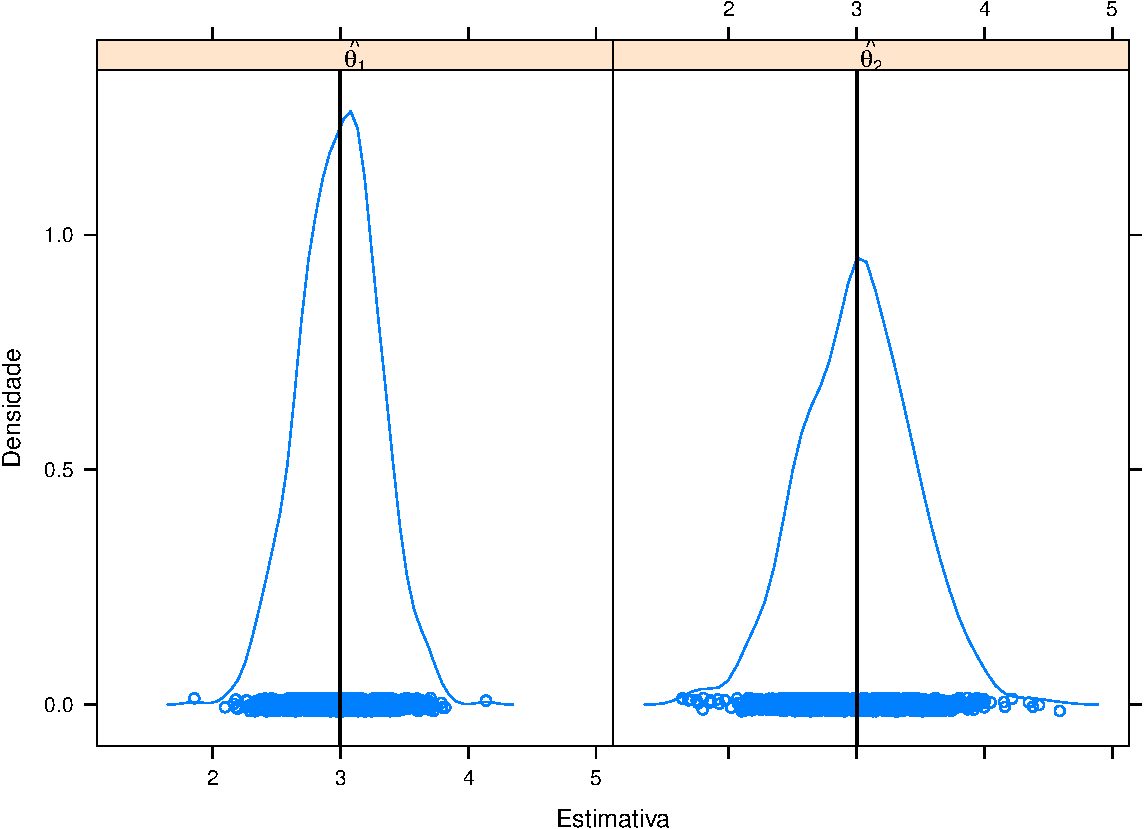
\includegraphics[width=1\textwidth]{vies_normal-crop}
  \end{figure}
\end{frame}

\begin{frame}[fragile]{Estimação pontual}{Pseudo-código 2 - $X \sim \N(3,1)$}
  \begin{figure}[h]
    \centering
    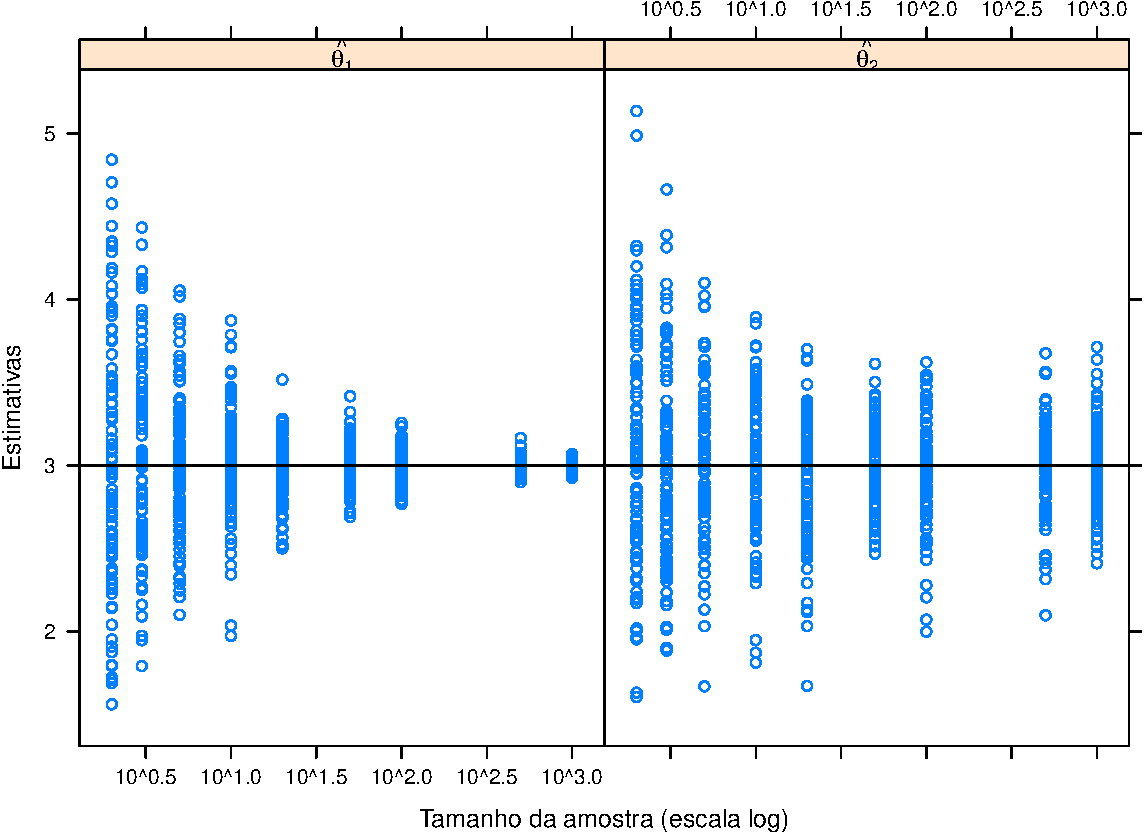
\includegraphics[width=1\textwidth]{consistencia_normal-crop}
  \end{figure}
\end{frame}

\begin{frame}[fragile]{Estimação pontual}
  \textbf{Exemplo 2:} Considere uma amostra aleatória ($X_1, \ldots,
  X_n$) de uma variável aleatória $Y \sim \text{U}(\text{min} = 2,
  \text{max} = 4)$ (distribuição uniforme no intervalo [2,4]) e os
  estimadores pontuais para $\mu$
  \begin{equation*}
    \hat{\theta}_1 = \frac{1}{n} \sum_{i=1}^n X_i \qquad \text{e} \qquad
    \hat{\theta}_2 = \frac{X_{(1)}+X_{(n)}}{2}
  \end{equation*}
  Qual dos dois estimadores pode ser considerado como o \textbf{melhor}
  para estimar a média de $Y$? \\~\\
\end{frame}

\begin{frame}[fragile]{Estimação pontual}{Pseudo-código 1 - $Y \sim \text{U}(2,4)$}
  \begin{figure}[h]
    \centering
    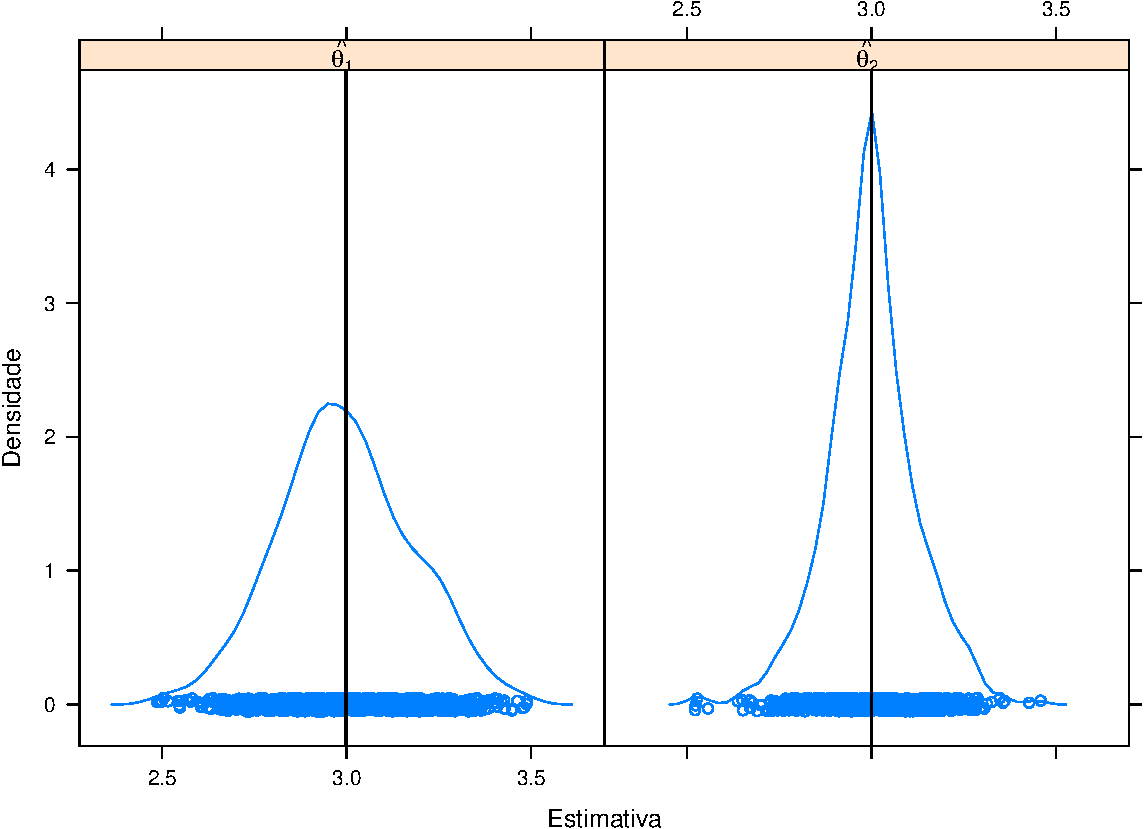
\includegraphics[width=1\textwidth]{vies_uniforme-crop}
  \end{figure}
\end{frame}

\begin{frame}[fragile]{Estimação pontual}{Pseudo-código 2 - $Y \sim \text{U}(2,4)$}
  \begin{figure}[h]
    \centering
    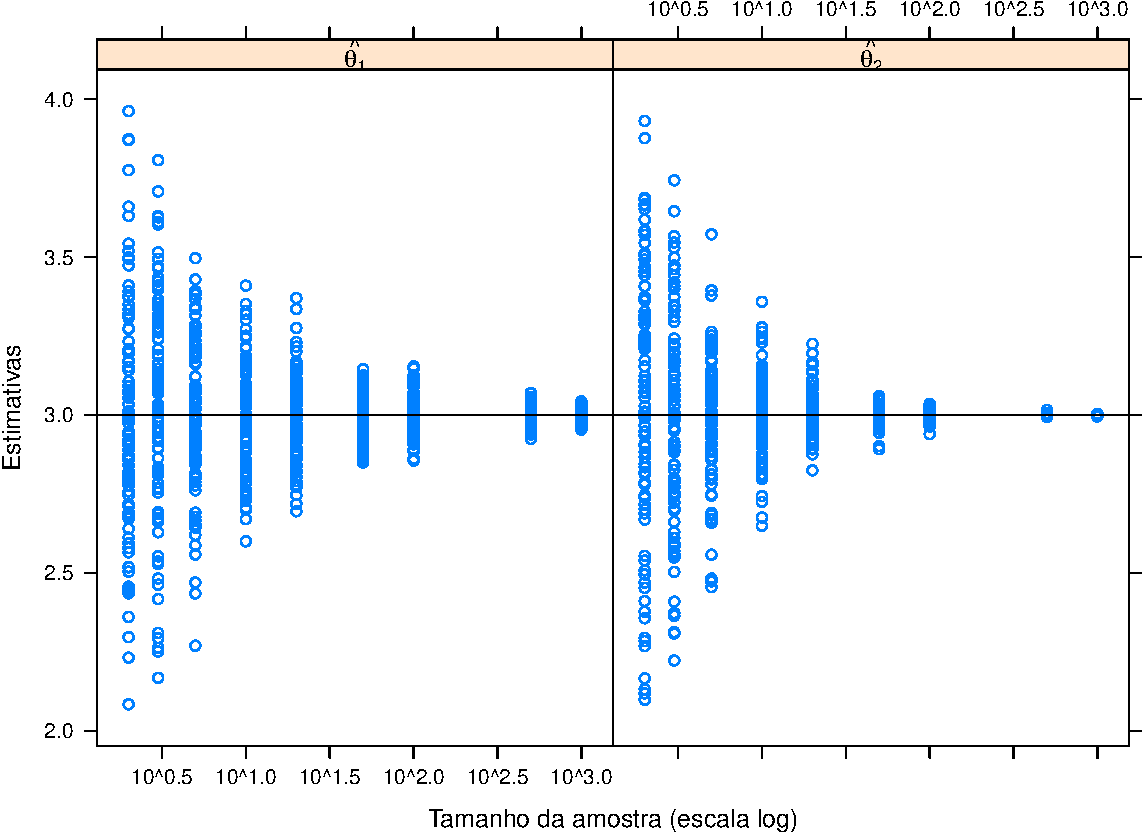
\includegraphics[width=1\textwidth]{consistencia_uniforme-crop}
  \end{figure}
\end{frame}

\subsection[Propriedades]{Propriedades dos estimadores}

\begin{frame}[fragile]{Propriedades dos estimadores}
  De modo geral, um ``\textbf{bom}'' estimador deve ser \\~\\
  \begin{enumerate}
%  \item Suficiente
  \item Não viciado
  \item Consistente
  \item Eficiente
  \end{enumerate}
\end{frame}

% \begin{frame}[fragile]{Propriedades dos estimadores}{1) Suficiência}
%   \begin{mydef}[Estimador suficiente]
%     Se $\hat{\theta} = T(\mb{X})$ é uma função de uma estatística
%     suficiente para $\theta$, então $\hat{\theta}$ é suficiente para
%     $\theta$, pelo princípio da equivalência.
%   \end{mydef}
% \end{frame}

\begin{frame}[fragile]{Propriedades dos estimadores}{1) Não viciado}
  \begin{mydef}[Erro quadrático médio (EQM)]
    O Erro Quadrático Médio (EQM) de um estimador $\hat{\theta}$ de
    $\hat{\theta}$ é dados por
    \begin{align*}
      \text{EQM}[\hat{\theta}] &= \E[(\hat{\theta} - \theta)^2] \\
                             &= \Var[\hat{\theta}] + \text{B}[\hat{\theta}]^2
    \end{align*}
    onde
    \begin{equation*}
      \text{B}[\hat{\theta}] = \E[\hat\theta] - \theta
    \end{equation*}
    é denominado de \textbf{vício} do estimador $\hat\theta$. Portanto,
    dizemos que um estimador é \textbf{não viciado} para $\theta$ quando
    \begin{equation*}
      \text{B}[\hat{\theta}] = 0 \quad \Rightarrow \quad \E[\hat{\theta}] = \theta
    \end{equation*}
  \end{mydef}
\end{frame}

\begin{frame}[fragile]{Propriedades dos estimadores}{1) Não viciado}
  \begin{mydef}[Estimador não viciado]
    Seja $(X_1, \ldots, X_n)$, uma amostra aleatória de uma variável
    aleatória com fdp ou fp $f(x,\theta)$, $\theta \in \Theta$, dizemos
    que o estimador $\hat{\theta} = T(\mb{X})$ é não viciado para
    $\theta$ se
    \begin{equation*}
      \E[\hat{\theta}] = \E[T(\mb{X})] = \theta \qquad \forall \, \theta
      \in \Theta
    \end{equation*}
  \end{mydef}
  Um estimador $\hat\theta$ é dito \textbf{assintoticamente não viciado}
  se
  \begin{equation*}
    \lim_{n \to \infty} \E[\hat{\theta}] = \theta
  \end{equation*}
  Ou seja, para grandes amostras, $\hat\theta$ passa a ser imparcial.
\end{frame}

\begin{frame}[fragile]{Propriedades dos estimadores}{2) Consistente}
  \begin{mydef}[Estimador consistente]
    Seja $(X_1, \ldots, X_n)$, uma amostra aleatória de uma variável
    aleatória com fdp ou fp $f(x,\theta)$, $\theta \in \Theta$, o
    estimador $\hat{\theta} = T(\mb{X})$ é consistente para $\theta$ se
    satisfaz simultaneamente
    \begin{equation*}
      \lim_{n \to \infty} \E[\hat{\theta}] = \theta
    \end{equation*}
    e
    \begin{equation*}
      \lim_{n \to \infty} \Var[\hat{\theta}] = 0
    \end{equation*}
  \end{mydef}
\end{frame}

\begin{frame}[fragile]{Propriedades dos estimadores}{3) Eficiente}
  \begin{mydef}[Eficiência relativa]
    Sejam $\hat{\theta}_1 = T_1(\mb{X})$ e $\hat{\theta}_2 =
    T_2(\mb{X})$ dois estimadores pontuais \textbf{não viciados} para
    $\theta$. A eficiência relativa de $\hat{\theta}_1$ em relação a
    $\hat{\theta}_2$ é
    \begin{equation*}
      \text{ER}[\hat{\theta}_1, \hat{\theta}_2] = \frac{\Var[\hat{\theta}_1]}{\Var[\hat{\theta}_2]}
    \end{equation*}
  \end{mydef}
  \vspace{1em}
  Se:
  \begin{itemize}
  \item $\text{ER}[\hat{\theta}_1, \hat{\theta}_2] > 1$ $\Rightarrow$
  $\hat\theta_2$ é mais eficiente
  \item $\text{ER}[\hat{\theta}_1, \hat{\theta}_2] < 1$ $\Rightarrow$
  $\hat\theta_1$ é mais eficiente
  \end{itemize}
\end{frame}

\begin{frame}[fragile]{Propriedades dos estimadores}
  \textbf{Exemplo}: média amostral $\bar{X} = \frac{1}{n} \sum_{i=1}^{n}
  X_i$ como estimador da média populacional $\mu$: \\~\\
  \begin{flalign*}
    \E(\bar{X}) &= \E \left[ \frac{1}{n} \sum_{i=1}^{n} X_i \right] = \mu&& \\
    \Var(\bar{X}) &= \Var \left[ \frac{1}{n} \sum_{i=1}^{n} X_i \right] = \frac{\sigma^2}{n}&&
  \end{flalign*}
  \vspace{1em}

  Portanto $\bar{X}$ é um estimador \textbf{não viciado} e
  \textbf{consistente} para $\mu$.
\end{frame}

\begin{frame}[fragile]{Propriedades dos estimadores}
  \textbf{Exemplo}: variância amostral $\hat{\sigma}^2 = \frac{1}{n}
  \sum_{i=1}^{n} (X_i - \bar{X})^2$ como estimador da variância populacional
  $\sigma^2$:
  \begin{flalign*}
    \E(\hat{\sigma}^2) = \E \left[ \frac{1}{n} \sum_{i=1}^{n} (X_i - \bar{X})^2 \right]
    = \left( \frac{n-1}{n} \right) \sigma^2 &&
  \end{flalign*}
  Portanto $\hat{\sigma}^2$ é um estimador \textbf{viciado} para
  $\sigma^2$. (Embora seja um estimador \textbf{assintoticamente} não
  viciado). \\~\\
  Para eliminar esse vício, podemos definir então um novo
  estimador: $s^2 = \frac{1}{n-1} \sum_{i=1}^{n} (X_i - \bar{X})^2$, e
  \begin{flalign*}
    \E(s^2) = \E \left[ \frac{1}{n-1} \sum_{i=1}^{n} (X_i - \bar{X})^2 \right]
    = \sigma^2 &&
  \end{flalign*}
  que é então um estimador \textbf{não viciado} para $\sigma^2$.
\end{frame}

\begin{frame}[fragile]{Propriedades dos estimadores}
  O \textbf{erro padrão} de um estimador dá uma ideia da
  \textbf{precisão} da estimativa.
  \begin{mydef}[Erro padrão de um estimador]
    O erro padrão (EP) de um estimador é o seu desvio-padrão (raíz
    quadrada da variância), ou seja,
    \begin{equation*}
      \EP(\hat\theta) = \sqrt{\Var(\hat\theta)}
    \end{equation*}
  \end{mydef}
  \vspace{1em}
  \textbf{Exemplo:} Sabemos que a distribuição de $\bar{X}$ tem
  média $\mu$ e variância $\sigma^2/n$. Então o erro padrão de $\bar{X}$ é
  \begin{equation*}
    \EP(\bar{X}) = \sqrt{\Var(\bar{X})} = \sqrt{\frac{\sigma^2}{n}} = \frac{\sigma}{\sqrt{n}}
  \end{equation*}
\end{frame}

\section{Erros amostrais}

\begin{frame}{Erros amostrais}
  \begin{block}{Erros amostrais}
    Diferença entre o resultado da amostra e o verdadeiro valor da
    população. Ocorre pois as amostras são \textbf{aleatórias}! \\
    \textbf{Exemplo}: a diferença entre a média amostral $\bar{X}$ e a
    média populacional $\mu$
    \begin{equation*}
      e = \bar{X} - \mu
    \end{equation*}
    é chamada de \textit{erro amostral da média}.
  \end{block}
  \vspace{1em}
  \begin{block}{Erros não amostrais}
    Ocorre quando os dados amostrais são coletados
    \textbf{incorretamente}, devido a uma \textsl{amostra tendenciosa},
    instrumento de medida defeituoso, anotações erradas, \ldots
  \end{block}
  \pause
  \begin{alertblock}{Atenção!}
    Os erros não amostrais não devem existir, ou devem ser minimizados
  \end{alertblock}
\end{frame}

\begin{frame}{Erros amostrais}
  Não importa quão bem a amostra seja coletada, os \textbf{erros
    amostrais} sempre irão ocorrer\\~\\
  Cada vez que uma amostra aleatória for retirada de uma população, um
  resultado diferente será observado\\~\\
  Selecione uma amostra de tamanho $n = 5$ das idades dos estudantes de
  uma sala: \texttt{22 21 24 23 20 22 21 25 24 24 23 19
    25 24 23 23 20 21 23 20 23
    22 23 23 25 25 20 23 24 20}\\~\\
  Repita 5 vezes (tente ser o mais aleatório possível!), calcule a média
  de cada amostra, e compare com a média populacional $\mu = 22,5$
\end{frame}


\begin{frame}{Um exemplo}
  \begin{table}[h]
    \centering
    \begin{tabular}{lrr}
      \hline
      Amostra & $\bar{x}$ & $e = \bar{x} - \mu$ \\
      \hline
      23 23 23 24 23 & 23.2 & 0.7 \\
      24 22 20 20 20 & 21.2 & -1.3 \\
      21 20 19 22 25 & 21.4 & -1.1 \\
      22 23 25 20 22 & 22.4 & -0.1 \\
      21 20 22 24 20 & 21.4 & -1.1 \\
      \hline
    \end{tabular}
  \end{table}
  \begin{itemize}
  \item O que isso nos diz a respeito das médias amostrais?
  \item O que isso nos diz a respeito da variabilidade das médias
    amostrais?
  \item E se fizemos uma ``\underline{média das médias}'' de todas as
    amostras?
  \end{itemize}
\end{frame}

\section{Distribuições amostrais}

\begin{frame}[fragile=singleslide]{Distribuições amostrais}
  Suponha que vamos retirar uma amostra de $n = 100$ indivíduos de uma
  população \\~\\
  Se selecionarmos aleatoriamente um indivíduo desta população, ele terá
  apenas um valor, $x_1$, de todos os possíveis valores da variável
  aleatória $X_1$ \\~\\
  Da mesma forma, um segundo indivíduo amostrado aleatoriamente terá o
  valor $x_2$ da variável aleatória $X_2$, e assim sucessivamente até o
  centésimo indivíduo amostrado com valor $x_{100}$ da variável
  aleatória $X_{100}$
\end{frame}

\begin{frame}[fragile=singleslide]{Distribuições amostrais}
  De maneira geral, uma amostra de tamaho $n$ será descrita pelos
  valores $x_1, x_2, \ldots, x_n$ das variáveis aleatórias $X_1, X_2,
  \ldots, X_n$ $\Rightarrow$ \textbf{Amostra Aleatória} \\~\\
  No caso de uma Amostragem Aleatória Simples (AAS) \textbf{com
    reposição}, $X_1, X_2, \ldots, X_n$ serão
  variáveis aleatórias \textbf{independentes e identicamentes
    distribuídas} (iid) com função de probabilidade (fp) ou função
  densidade de probabilidade (fdp) $f(x)$ \\~\\
  Isto significa que quando observamos cada amostra $x_i$ de uma
  população indexada por um parâmetro $\bs{\theta}$ (um escalar ou um
  vetor), então cada observação possui fp ou fdp dada por $f(x,
  \bs{\theta})$
\end{frame}

\begin{frame}[fragile=singleslide]{Distribuições amostrais}
  Se somente uma observação $X$ é feita, então as probabilidades
  referentes a $X$ podem ser calculadas diretamente utilizando
  $f(x,\bs{\theta})$ \\~\\
  No entanto, na maioria das vezes temos $n>1$ observações de $X$. Como
  vimos que as variáveis $X_i$ são iid, temos que a fp ou fdp conjunta
  será
  \begin{equation*}
    f(x_1, x_2, \ldots, x_n, \bs{\theta}) = f(x_1,\bs{\theta}) \cdot
    f(x_2,\bs{\theta}) \cdots f(x_n,\bs{\theta}) = \prod_{i=1}^{n}
    f(x_i,\bs{\theta})
  \end{equation*}
  Onde o mesmo valor do parâmetro $\bs{\theta}$ é utilizado em cada um dos
  termos no produto
\end{frame}

\begin{frame}[fragile=singleslide]{Distribuições amostrais}
  \begin{block}{Exemplo: distribuição conjunta da Bernoulli($\pi$)}
    Para uma observação, temos que a fp da Bernoulli($\pi$) é
    \begin{equation*}
      f(x,\pi) = \pi^x (1-\pi)^{1-x} \mathbb{I}_{\{0,1\}}(x)
    \end{equation*}
    Para uma amostra aleatória $X_1, X_2, \ldots, X_n$
    \begin{align*}
      f(\mb{x},\pi) &= \prod_{i=1}^{n} \pi^{x_{i}} (1-\pi)^{1-x_{i}}
      \mathbb{I}_{\{0,1\}}(x_i) \\
      &= \pi^{\sum_{i=1}^{n} x_i} (1-\pi)^{n - \sum_{i=1}^{n} x_i}
      \prod_{i=1}^{n} \mathbb{I}_{\{0,1\}}(x_i)
    \end{align*}
  \end{block}
\end{frame}

\begin{frame}[fragile=singleslide]{Distribuições amostrais}
  Quando uma amostra $X_1, X_2, \ldots, X_n$ é obtida, geralmente
  estamos interessados em um resumo destes valores, que pode ser
  expresso matematicamente pela estatística $T(x_1, x_2, \ldots, x_n)$
  \\~\\
  A função $T(\cdot)$ pode ser um valor real ou um vetor. Dessa forma,
  $Y = T(x_1, x_2, \ldots, x_n)$ \textbf{é também uma variável
    aleatória} (ou vetor aleatório). Se $Y$ é uma VA, \emph{então ela possui
  uma distribuição de probabilidade}. \\~\\
  Uma vez que a amostra aleatória $X_1, X_2, \ldots, X_n$ tem uma
  estrutura probabilística simples (porque $X_i$ são iid), $Y$ é
  particularmente tratável. Uma vez que a distribuição de $Y$ é derivada
  desta estrutura, vamos denominá-la de \textbf{distribuição amostral}
  de $Y$.
\end{frame}

\begin{frame}[fragile=singleslide]{Distribuições amostrais}
  \begin{mydef}[Distribuição amostral]
    A distribuição de probabilidade de uma estatística $Y = T(x_1, x_2,
    \ldots, x_n)$ é denominada de \textbf{distribuição amostral} de
    $Y$. Assim, uma estatística também é uma variável aleatória, pois
    seus valores mudam conforme a amostra aleatória
  \end{mydef}
  \vspace{1em}
    \textbf{Exemplo}: duas estatísticas comumente utilizadas para o
    resumo de uma amostra aleatória são a \textbf{média amostral}
\begin{equation*}
  \bar{X} = \frac{1}{n} \sum_{i=1}^{n} X_i
\end{equation*}
e a \textbf{proporção amostral}
\begin{equation*}
  \hat{p} = \frac{x}{n}
\end{equation*}
\end{frame}

\subsection{Distribuição amostral da média}

\begin{frame}[fragile=singleslide]{Distribuição amostral da média}
  Para estudarmos a distribuição amostral da estatística $\bar{X}$,
  considere uma população identificada pela VA $X$, com parâmetros
  \begin{equation*}
    \E(X) = \mu = \text{média} \qquad \qquad \Var(X) = \sigma^2 =
    \text{variância}
  \end{equation*}
  supostamente conhecidos. Em seguida, realizamos os seguintes passos:
  \begin{enumerate}
  \item Retiramos $m$ amostras aleatórias (AAS com reposição) de tamanho
    $n$ dessa população
  \item Para cada uma das $m$ amostras, calculamos a média amostral
    $\bar{x}$
  \item Verificamos a distribuição das $m$ médias amostrais e estudamos
    suas propriedades
  \end{enumerate}
\end{frame}

\begin{frame}{Voltando ao exemplo \ldots}
  \begin{table}[h]
    \centering
    \small
    \begin{tabular}{lrr}
      \hline
      Amostra & $\bar{x}$ & $\epsilon = \bar{x} - \mu$ \\
      \hline
      23 23 23 24 23 & 23.2 & 0.7 \\
      24 22 20 20 20 & 21.2 & -1.3 \\
      21 20 19 22 25 & 21.4 & -1.1 \\
      22 23 25 20 22 & 22.4 & -0.1 \\
      21 20 22 24 20 & 21.4 & -1.1 \\
      \hline
    \end{tabular}
  \end{table}
  \begin{figure}[h]
    \centering
    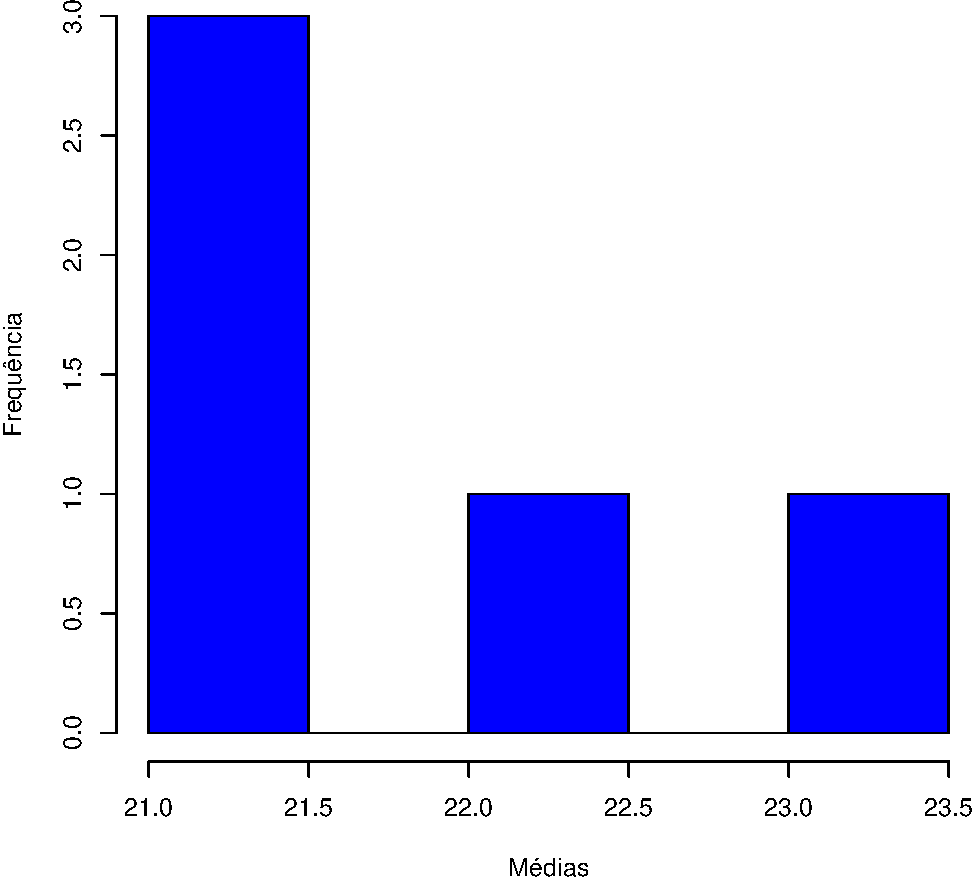
\includegraphics[width=.5\textwidth]{hist-crop}
  \end{figure}
\end{frame}

\begin{frame}{Voltando ao exemplo \ldots}
  Do exemplo anterior, temos que $\mu = 22,5$, e $\sigma^2 = 3,09$\\~\\
  Para esta tabela, com $m=5$ e $n=5$:
  \begin{itemize}
  \item A \underline{média das médias} é $\mu_{\bar{X}} = 21,9$
  \item A \underline{variância das médias} é $\sigma^2_{\bar{X}} = 0,732$
  \end{itemize}
\end{frame}

\begin{frame}[fragile=singleslide]{Distribuição amostral da média}
  E se pudessemos retirar \textbf{todas} as amostras \textbf{com
    reposição} de tamanho $n=5$ dessa população??? \\~\\
  Teriamos que fazer $N^n = 20^5 = 3.200.000$ amostragens! \\~\\
  Para $n=10$ $\Rightarrow$ $N^n = 20^{10} = 1,024 \times 10^{13}$ \\~\\
  Para $n=15$ $\Rightarrow$ $N^n = 20^{15} = 3,2768 \times 10^{19}$ \\~\\
  O computador pode fazer isso, e o resultado é (para $n=15$)
  \begin{itemize}
  \item $\mu_{\bar{X}} = 22,5$
  \item $\sigma^2_{\bar{X}} \approx 0,2 = \sigma^2/n \approx 3,09/15$
  \end{itemize}
  \vspace{1em}
  \textbf{Conclusão}:
  \begin{itemize}
  \item A média de \textbf{todas} as médias é igual à média da
    população!
  \item A variância das médias é menor porque a variabilidade
    entre as médias é menor!
  \end{itemize}
\end{frame}

\begin{frame}{Voltando ao exemplo \ldots}
Veja a figura \texttt{dist\_amostral\_idades.pdf}\\~\\
\begin{itemize}
\item O primeiro gráfico é a distribuição da população original
\item O segundo gráfico é a distribuição de 1000 médias, calculadas a
  partir de 1000 amostras de tamanho 5 ($m=1000$ e $n=5$)
\item Os demais gráficos mostram a distribuição amostral de 1000 médias
  calculadas com amostras de tamanho $n=10$ e $n=15$
\item Repare que:
  \begin{itemize}
  \item A distribuição das 1000 médias se torna cada vez mais próxima de
    uma normal, conforme o tamanho da amostra aumenta
  \item A variabilidade da distribuição amostral das médias diminui
    conforme o tamanho da amostra aumenta
  \item A distribuição amostral tende a se concentrar cada vez mais em
    torno da média populacional verdadeira
  \end{itemize}
\end{itemize}
\end{frame}

\begin{frame}[fragile=singleslide]{Distribuição amostral da média}
  Através do estudo da distribuição da média amostral chegamos em um dos
  resultados mais importantes da inferência estatística
  \begin{mythm}[Distribuição amostral da média]
    \begin{itemize}
    \item $\E(\bar{X}) = \mu_{\bar{X}} = \mu$
    \item $\Var(\bar{X}) = \sigma^2_{\bar{X}} = \sigma^2/n$
    \end{itemize}
  \end{mythm}
  Portanto, se
  \begin{equation*}
    X \sim \text{N}(\mu, \sigma^2) \quad \text{então} \quad
    \bar{X} \sim \text{N}(\mu_{\bar{X}}, \sigma^2_{\bar{x}})
  \end{equation*}
  mas, como
  \begin{equation*}
    \mu_{\bar{X}} = \mu \quad \text{e} \quad \sigma^2_{\bar{X}} = \sigma^2/n
  \end{equation*}
  então, a \textbf{distribuição amostral} da média amostral $\bar{X}$ é
  \begin{equation*}
    \bar{X} \sim \text{N}\left(\mu, \frac{\sigma^2}{n} \right)
  \end{equation*}
\end{frame}

\begin{frame}[fragile=singleslide]{Distribuição amostral da média}
  \begin{mythm}[Teorema Central do Limite (TCL)]
    Para amostras aleatórias simples $(X_1, X_2, \ldots, X_n)$,
    retiradas de uma população normal com média $\mu$ e variância
    $\sigma^2$, a distribuição amostral da média $\bar{X}$,
    terá forma dada por
    \begin{equation*}
      Z = \frac{\bar{X} - \mu}{\sigma/\sqrt{n}}
    \end{equation*}
    no limite quando $n \to \infty$, que é a ditribuição normal padrão:
    $Z \sim \N(0,1)$.
  \end{mythm}
  \begin{itemize}
  \item Se a população for normal, então $\bar{X}$ terá distribuição
    \textit{exata} normal.
  \item A rapidez da convergência para a normal depende da distribuição
    da população da qual as amostras foram geradas
  \end{itemize}
\end{frame}


\begin{frame}[fragile=singleslide]{Distribuição amostral da média}
  Este teorema nos mostra que, para amostras suficientemente grandes ($n
  > 30$), \textbf{a média amostral $\bar{X}$  converge para o verdadeiro
  valor da média populacional $\mu$} (é um \textbf{estimador
  não viesado} de $\mu$) \\~\\
  Além disso, a variância das médias amostrais $\sigma^2_{\bar{X}}$
  tende a diminuir conforme $n \rightarrow \infty$ (é um estimador
  \textbf{consistente}) \\~\\
  Estes resultados sugerem que, quando o tamanho da amostra aumenta,
  \begin{center}
  \underline{independente do formato da distribuição da população
    original},
  \end{center}
  \textbf{a distribuição amostral de $\bar{X}$ aproxima-se
    cada vez mais de uma distribuição normal}, um resultado fundamental
  na teoria de probabilidade conhecido como \textbf{Teorema Central do Limite}
\end{frame}

\begin{frame}{Distribuição amostral da média}
Exemplo computacional $\rightarrow$ veja a figura
\texttt{dist\_amostrais.pdf}
\end{frame}


% \begin{frame}{Distribuição amostral da média}
%   Outra forma de apresentar o TLC é através do resultado
%   \begin{equation*}
%     Z = \frac{\bar{X} - \mu}{\sigma/\sqrt{n}} \, \sim \, \text{N}(0,1)
%   \end{equation*}
%   que decorre da transformação usual de uma variável aleatória $X \sim
%   \text{N}(\mu, \sigma^2)$ para uma normal padrão $\text{N}(0,1)$,
%   \begin{equation*}
%     Z = \frac{X - \mu}{\sigma}
%   \end{equation*}
%   % Nesse caso, assumindo que $\sigma$ é conhecido, e $\bar{X}$ será
%   % medido, podemos usar $Z$ para estimar $\mu$
% \end{frame}

\begin{frame}{Distribuição amostral da média}
  Em palavras, o teorema garante que que para $n$ grande, a distribuição
  da média amostral, devidamente padronizada, \textbf{se comporta segundo um
  modelo normal} com média 0 e variância 1. \\~\\
  Pelo teorema, temos que quanto maior o tamanho da amostra, \textbf{melhor é a
  aproximação}. \\~\\
  Estudos envolvendo simulações mostram que, em muitos casos, \textbf{valores de
  $n$ ao redor de 30} fornecem aproximações bastante boas para as
  aplicações práticas.
\end{frame}

\begin{frame}{Distribuição amostral da média}
  Quando calculamos a probabilidade de um valor estar em um determinado
  intervalo de valores, podemos usar o modelo Normal, como vimos
  anteriormente. \\~\\
  No entanto, quando temos uma \textbf{amostra}, e queremos calcular
  probabilidades associadas à \textbf{média amostral} (a probabilidade
  da média amostral estar em um determinado intervalo de valores),
  precisamos necessariamente usar os resultados do TCL.
\end{frame}

\begin{frame}{Distribuição amostral da média e erros amostrais}
  Já vimos que o \textbf{erro amostral da média} é dado pela diferença
  entre $\bar{X}$ e $\mu$, ou seja,
  \begin{equation*}
    e = \bar{X} - \mu
  \end{equation*}
  Dessa forma, se
  \begin{equation*}
    Z = \frac{\bar{X} - \mu}{\sigma/\sqrt{n}} \, \sim \, \N(0,1)
  \end{equation*}
  então a distribuição de $e$ também será normal padrão, pois
  \begin{equation*}
    \frac{e \sqrt{n}}{\sigma} \, \sim \, \N(0,1)
  \end{equation*}
  Esse resultado será fundamental na construção de estimativas
  intervalares.
\end{frame}

\begin{frame}{Distribuição amostral da média}
  \textbf{Usando o TCL} \\~\\

  \textbf{Exemplo:} Uma máquina de empacotamento que abastece pacotes de
  feijão apresenta distribuição normal com média de 500 g e
  desvio-padrão de 22 g. De acordo com as normas de defesa do
  consumidor, os pacotes de feijão não podem ter peso inferior a 2\% do
  estabelecido na embalagem.
  \begin{itemize}
  \item[a)] Determine a probabilidade de \textbf{um pacote} selecionado
    aleatoriamente ter a peso inferior a 490 g.
  \item[b)] Determine a proabilidade de \textbf{20 pacotes} selecionados
    aleatoriamente terem peso médio inferior a 490 g.
  \item[c)] Como podemos interpretar os resultados dos itens anteriores?
    O que é mais indicado para se tomar uma decisão sobre o
    funcionamento da máquina: selecionar um pacote ou uma amostra?
  \end{itemize}
\end{frame}

\begin{frame}{Distribuição amostral da média}
  \textbf{Usando o TCL} \\~\\

  \textbf{Exemplo:} Uma pesquisa com 12000 estudantes mostrou que a
  média de horas de estudo por semana foi de 7,3 horas, com
  desvio-padrão de 4,2 horas. \textbf{O tempo de estudo não apresenta
    distribuição normal}. Com isso calcule:
  \begin{itemize}
  \item[a)] A probabilidade de que \textbf{um} estudante exceda 8 horas de
    estudo por semana.
  \item[b)] Dada uma amostra de 45 estudantes, a probabilidade de que o
    \textbf{tempo médio} de estudo exceda 8 horas por semana.
  \item[c)] Dada uma amostra de 45 estudantes, a probabilidade de que o
    \textbf{tempo médio} de estudo seja igual ou superior a 7 horas por
    semana.
  \end{itemize}
\end{frame}

\subsection{Distribuição amostral da proporção}

\begin{frame}{Distribuição amostral da proporção}
  Muitas vezes, o interesse é conhecer uma \textbf{proporção}, e não a
  média de uma população. \\~\\
  Suponha que uma amostra de tamanho $n$ foi obtida de uma população, e
  que $x \leq n$ observações nessa amostra pertençam a uma classe de
  interesse (ex.: pessoas do sexo masculino). \\~\\
  Dessa forma, a proporção amostral
  \begin{equation*}
    \hat{p} = \frac{x}{n} = \frac{\text{número de sucessos}}{\text{total de
        tentativas}}
  \end{equation*}
  é o ``melhor estimador'' para a proporção populacional $p$. \\~\\
  Note que $n$ e $p$ são os parâmetros de uma \textbf{distribuição
    binomial}.
\end{frame}

\begin{frame}{Distribuição amostral da proporção}
  \textbf{Exemplo}: em 5 lançamentos de uma moeda considere que o evento
  ``cara'' (C) seja o sucesso (``sucesso'' = 1; ``fracasso'' = 0). Um possível
  resultado seria o conjunto \{C, C, R, R, C\}. A proporção
  amostral seria
  \begin{equation*}
    \hat{p} = \frac{x}{n} = \frac{\text{número de sucessos}}{\text{total de
        tentativas}} = \frac{3}{5} = 0,6
  \end{equation*}
  \vspace{1em}

  \textbf{Exemplo}: em uma amostra de 2500 eleitores de uma cidade, 1784
  deles eram favoráveis à reeleição do atual prefeito. A proporção
  amostral é então
  \begin{equation*}
    \hat{p} = \frac{x}{n} = \frac{\text{número de sucessos}}{\text{total de
        tentativas}} = \frac{1784}{2500} = 0,7136
  \end{equation*}
\end{frame}


\begin{frame}{Distribuição amostral de uma proporção}
  A distribuição amostral de uma \textbf{proporção} é a distribuição das
  proporções de todas as possíveis amostras de tamanho $n$ retiradas de
  uma população \\~\\
  Ver figura \texttt{dist\_amostral\_proporcoes.pdf}:
  \begin{itemize}
  \item Uma moeda é lançada $n=10$ vezes, e a proporção de caras é
    registrada
  \item Esse processo é repetido $m = 10, 30, 100, 1000, 10000$ vezes
  \end{itemize}
  \vspace{1em}
  Com isso, concluimos que:
  \begin{itemize}
  \item A média das proporções para $m \to \infty$ tende para a
    verdadeira proporção populacional $p = 0,5$
  \item A \textbf{distribuição amostral} das proporções segue
    aproximadamente uma \textbf{distribuição normal}
  \end{itemize}
\end{frame}

\begin{frame}{Distribuição amostral de uma proporção}
  Através do estudo da distribuição amostral da proporção, chegamos aos
  seguintes resultados
  \begin{itemize}
  \item $\E(\hat{p}) = \mu_{\hat{p}} = p$
  \item $\Var(\hat{p}) = \sigma^{2}_{\hat{p}} = \frac{p(1-p)}{n}$
  \end{itemize}
  \vspace{1em}

  Ou seja, $\hat{p}$ é um estimador \textbf{não viciado} e
  \textbf{consistente} para $p$. \\~\\
  Assim, a \textbf{distribuição amostral} de $\hat{p}$ será
  \begin{equation*}
    \hat{p} \sim \N \left( p, \frac{p(1-p)}{n} \right)
  \end{equation*}
\end{frame}

\begin{frame}{Distribuição amostral de uma proporção}
  Note que o \textbf{erro padrão} de $\hat{p}$ será
  \begin{equation*}
    \EP(\hat{p}) = \sqrt{\Var(\hat{p})} = \sqrt{\frac{p(1-p)}{n}}
  \end{equation*}
  Assim, usando o TCL, podemos mostrar que a quantidade
  \begin{equation*}
    Z = \frac{\hat{p} - p}{\sqrt{\frac{p(1-p)}{n}}} \, \sim \, \N(0,1)
  \end{equation*}
  segue uma distribuição \textbf{normal padrão} com média 0 e variância
  1. \\~\\
  Quando não conhecemos $p$, usamos $\hat{p} = x/n$ como estimativa para
  calcular o erro padrão.
\end{frame}

\begin{frame}{A normal como aproximação da binomial}
  Sob determinadas condições, podemos usar a distribuição normal como
  aproximação da distribuição binomial. \\~\\
  Se $X$ for uma VA binomial com parâmetros $n$ e $p$, então
  \begin{equation*}
    Z = \frac{X - np}{\sqrt{np(1-p)}}
  \end{equation*}
  será uma VA \textbf{normal padrão}, $Z \sim \N(0,1)$, desde que as
  seguintes condições sejam satisfeitas:
  \begin{itemize}
  \item $np \geq 5$
  \item $n(1-p) \geq 5$
  \end{itemize}
  Dessa forma, podemos calcular probabilidades para uma VA binomial,
  aproximadas por uma distribuição normal com média $\mu = np$ e
  desvio-padrão $\sigma = \sqrt{np(1-p)}$.
\end{frame}

\section{Referências}

\begin{frame}{Referências}
  \begin{itemize}
  \item Bussab, WO; Morettin, PA. \textbf{Estatística básica}. São
    Paulo: Saraiva, 2006. [Cap. 10]
  \item Magalhães, MN; Lima, ACP. \textbf{Noções de Probabilidade e
      Estatística}. São Paulo: EDUSP, 2008. [Cap. 7]
  \item Montgomery, DC; Runger, GC. \textbf{Estatística aplicada e
      probabilidade para engenheiros}. Rio de Janeiro: LTC Editora,
    2012. [Cap. 7]
  \end{itemize}
\end{frame}

\end{document}
